\documentclass[preview]{standalone}
\usepackage{tikz}
\usetikzlibrary{decorations.pathmorphing, shapes.geometric}

% Definición de colores personalizados
\definecolor{primaryColor}{RGB}{20,45,105} % color primario
\definecolor{secondaryColor}{RGB}{0,100,160} % Color secundario

\begin{document}
% ============================================================================
% SLIDE 5: Colisiones de Protones \& Hard Scattering
% ============================================================================
            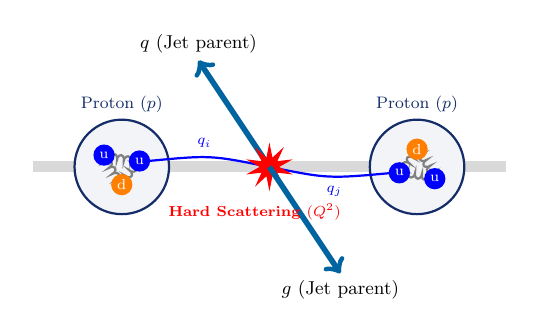
\begin{tikzpicture}[scale=0.75, transform shape]
                % Haz de Protones (Fondo del acelerador)
                \draw[gray!30, line width=4pt] (-4,0) -- (4,0);
                
                % Protón Izquierdo (Estructura interna)
                \draw[thick, primaryColor, fill=primaryColor!5] (-2.5,0) circle (0.8cm);
                \node[above, primaryColor] at (-2.5,0.8) {\footnotesize Proton ($p$)};
                % Intercambio de gluones interno (Densely Dashed = Seguro y limpio)
                \draw[thick, gray, decoration={coil, amplitude=1pt, segment length=2.5pt}, decorate] (-2.8,0.2) -- (-2.2,0.1);
                \draw[thick, gray, decoration={coil, amplitude=1pt, segment length=2.5pt}, decorate] (-2.2,0.1) -- (-2.5,-0.3);
                \draw[thick, gray, decoration={coil, amplitude=1pt, segment length=2.5pt}, decorate] (-2.8,0.2) -- (-2.5,-0.3);
                % quarks
                \fill[blue] (-2.8,0.2) circle (0.18) node[white]{\scriptsize u};
                \fill[blue] (-2.2,0.1) circle (0.18) node[white]{\scriptsize u};
                \fill[orange] (-2.5,-0.3) circle (0.18) node[white]{\scriptsize d};
                
                % Protón Derecho (Estructura interna)
                \draw[thick, primaryColor, fill=primaryColor!5] (2.5,0) circle (0.8cm);
                \node[above, primaryColor] at (2.5,0.8) {\footnotesize Proton ($p$)};
                % Intercambio de gluones interno (Densely Dashed = Seguro y limpio)
                \draw[thick, gray, decoration={coil, amplitude=1pt, segment length=2.5pt}, decorate] (2.8,-0.2) -- (2.2,-0.1);
                \draw[thick, gray, decoration={coil, amplitude=1pt, segment length=2.5pt}, decorate] (2.2,-0.1) -- (2.5,0.3);
                \draw[thick, gray, decoration={coil, amplitude=1pt, segment length=2.5pt}, decorate] (2.8,-0.2) -- (2.5,0.3);
                % quarks
                \fill[blue] (2.8,-0.2) circle (0.18) node[white]{\scriptsize u};
                \fill[blue] (2.2,-0.1) circle (0.18) node[white]{\scriptsize u};
                \fill[orange] (2.5,0.3) circle (0.18) node[white]{\scriptsize d};
                
                % Líneas de los partones interactuantes hacia el centro
                \draw[thick, ->, blue] (-2.05,0.1) .. controls (-1,0.2) .. (0,0);
                \draw[thick, ->, blue] (2.1,-0.1) .. controls (1,-0.2) .. (0,0);
                \node[above, blue] at (-1.1,0.2) {\scriptsize $q_i$};
                \node[below, blue] at (1.1,-0.2) {\scriptsize $q_j$};
                
                % Estado final saliente (Partones de alto pT)
                \draw[line width=2pt, ->, secondaryColor] (0,0) -- (-1.2,1.8);
                \node[above, black] at (-1.2,1.8) {\small $q$ (Jet parent)};
                
                % Punto de Interacción (Hard Scattering)
                \node[star, star points=10, star point ratio=2.5, fill=red, minimum size=0.8cm] at (0,0) {};
                

                \draw[line width=2pt, ->, secondaryColor] (0,0) -- (1.2,-1.8);
                \node[below, black] at (1.2,-1.8) {\small $g$ (Jet parent)};

                \node[below=0.4cm, red] at (-0.25,-0.1) {\scriptsize \textbf{Hard Scattering} ($Q^2$)};
            \end{tikzpicture}
\end{document}